\documentclass[a4paper, 10pt, notitlepage]{article}

\usepackage{moreverb} %para importar codigo

\usepackage{pepotina} %paquete personal para la caratula del DC

\usepackage[spanish,activeacute]{babel}
\usepackage{babel} %paquete de idioma

\usepackage[latin1]{inputenc}

%\usepackage{color}

\usepackage{hyperref}
%\usepackage[all]{hypcap}

\usepackage{caeycaeING}

\usepackage{fancyhdr} %linea sup con comentarios

\usepackage{lscape} %para hoja apaisada

\usepackage{framed} %para crear cajas de texto

\usepackage{lastpage} %ultima pagina

%\usepackage{pstricks}
%\usepackage{uml} %UML

\usepackage{listings}
%\lstset{
%  breaklines=true,                                     % line wrapping on
%  language=ocl,
%  frame=ltrb,
%  framesep=5pt,
%  basicstyle=\normalsize,
%  keywordstyle=\ttfamily\color{OliveGreen},
%  identifierstyle=\ttfamily\color{CadetBlue}\bfseries,
%  commentstyle=\color{Brown},
%  stringstyle=\ttfamily,
%  showstringspaces=ture
%}

\addtolength{\topmargin}{-50pt} 
\addtolength{\textwidth}{105pt}
\addtolength{\textheight}{120pt}
\addtolength{\oddsidemargin}{-50pt}

%\newcommand{\minix}{\textsl{minix }}

%%% Encabezado y pie de p'agina
\pagestyle{fancy}
\fancyhead[LO]{Ingenieria del Software I}
\fancyhead[C]{}
\fancyhead[RO]{P\'agina \thepage\ de \pageref{LastPage}}
\renewcommand{\headrulewidth}{0.4pt}
\fancyfoot{}

\newcommand{\depto}{{\bf DPTO: }}


\def\falta#1{ \begin{framed}	\begin{center} \hspace{1cm} \Large FALTA \normalsize #1 \hspace{1cm} \end{center} \end{framed}}


\def\imagen#1#2#3{\vskip0.5cm
{\large #3}
\begin{center}
\includegraphics[scale=#1]{#2}
\end{center}}


\begin{document}

\universidad{Universidad de Buenos Aires}
\facultad{Facultad de ciencias exactas y naturales}
\departamento{Departamento de Computacion}
\materia{Ingenieria del Software I}
\resumen{Proyecto casino online}
\keys{UML, Objetivos, Agentes, Casos De Uso, Diagrama De Contexto, Modelo Conceptual, OCL, Diagrama de Actividades, FSM}
\titulo{Proyecto: Casino Online}
\subtitulo{Informe 1: Analisis de Requerimientos y especificaci�n}
\grupo{Numero de grupo: 2}
\fecha{1er Cuatrimeste 2008}
\footspace{1cm}
\integrante{Aquino, Isis}{313/05}{isisaquino@yahoo.com.ar}
\integrante{Alvarez, Maria de los Angeles}{264/05}{mdelosaalvarez@hotmail.com}
\integrante{Engler, Christian Alejandro}{314/05}{caeycae@gmail.com}

%caratula
\maketitle{}

\tableofcontents

\newpage

\section{Introducci�n}


\section{Introduccion}
\newpage

\section{Vista Modular}
\label{sec:VistaModular}

Para organizar el dise�o, dividimos el problema en varios problemas independientes con el fin de hacer el dise�o mas flexible y con espectativas de ocultamiento por capas, de modo de que a cada capa se le pudiera cambiar la implementacion.

\subsection{Modulos Server}

\imagen{0.70}{img/componentes.png}{Vista Modular Server}

\newpage
\paragraph{Descripcion de cada uno de los modulos}
\label{sec:DescripcionDeCadaUnoDeLosModulos}

\begin{description}
	\item[Mensajero] El modulo mensajero se ocupa de recibir los mensajes que le envian los clientes al servidor del casino online. Sus obligaciones son ``chequear'' la llegada de un mensaje, empaquetarlo y entregarselo al siguiente modulo.
	\item[Interprete] El modulo interprete se ocupa de tomar un mensaje e intentar trasformarlo a un lenguaje entendible por los servicios del casino, en caso de que el mensaje no corresponda al formato esperado, debera notificar al cliente. Para lograr esta transformacion hace uso del modulo Parser.
	\item[Parser] Este modulo convierte los datos del lenguaje de comunicacion al lenguaje que maneja el casino y viceversa. Esto es para que la eleccion del lenguaje de cada una de estas partes sea independiente y no afecte al resto del sistema.
	\item[Servicios] Este modulo nuclea todos los servicios que presenta el casino. El dise�o del casino esta ocultado detras de este modulo para que la implementacion de estos servicios pueda ser modificada sin grandes efectos colaterales.
	\item[Casino] Aqui esta el casino propiamente dicho, independiente a toda forma de comunicacion y protocolo. Este modulo se encarga de realizar todo lo especificado en el informe I.
\end{description}
\newpage

\subsection{Modulos Cliente y Administrador}

\imagen{0.60}{img/componentesCliente.png}{Vista Modular Cliente}

\newpage

\section{Modulos}
\label{sec:Modulos}

\subsection{Mensajero / Interpretador}
\label{sec:MensajeroInterpretador}

Dise�amos un servicio ``core'' de mensajeria para que administre la recepcion de mensajes independientemente del uso que se le de a ellos.\\
Presentamos aqui un diagrama de secuencia con un ejemplo de uso correcto del servicio de mensajeria.
No nos comprometemos a que la implementacion del servicio sea ``porArchivos'', pero respetar� el modelo propuesto por la clase abstracta mensajero.
\imagen{0.45}{img/mensajeroSeq.png}{Diagrama de Secuencia: Mensajero}
\newpage

Ahora veamos mas en particular la operacion \textbf{OnMessage}. Esta operacion invoca al listener asociado al mensajero, dicha clase dira al mensajero que operacion realizar en el momento de recibir un mensaje.
\imagen{0.45}{img/onMessageSeq.png}{Diagrama de Secuencia: OnMessage}
\newpage

Para completar la explicacion del dise�o de este modulo necesitamos el diagrama de clases.

\imagen{0.50}{img/mensajeroInterpretador.png}{Diagrama de Clases: Mensajero / Interpretador}
\newpage

\subsection{Interpretador / Parser / Servicios}

No hay mucha complejidad en estas interacciones y estan suficientemente ilustradas en el diagrama de secuencia anterior. Presentamos el diagrama de clases de los modulos restantes.

\imagen{0.50}{img/interpretadorServicios.png}{Diagrama de Clases: Interpretador / Parser / Servicios}
\newpage

\subsection{Casino}

\imagen{0.40}{img/CasinoJugadorInvitadoClases.PNG}{Diagrama de Clases: Casino / Jugador / Invitado / TipoJugada}
\newpage

\imagen{0.40}{img/TragamonedasClases.PNG}{Diagrama de Clases: Traga}
\newpage

\imagen{0.40}{img/CrapsClases.PNG}{Diagrama de Clases: Craps}
\newpage

\imagen{0.40}{img/MensajesClases.PNG}{Diagrama de Clases: Mensajes}
\newpage

\section{Funcionalidad Casino}
\label{sec:FuncionalidadCasino}

\subsection{Registracion y Ingreso al casino online y modificacion de saldo}

\subsubsection{Registracion}

Segun lo acordado en la especificacion, la registracion de los usuarios se hace por fuera del sistema informatico del casino online.\\
En el momento de abrir el casino el sistema contar� con un archivo XML (en el futuro podria ser de otra manera)
\\
\textbf{Dicho archivo tendr� la siguiente sintaxis:}

\begin{framed}
\begin{verbatim}
<jugadores>
    <jugador nombre="Nombre" saldo"valor numerico del saldo" vip="true | false">
</jugadores>
\end{verbatim}
\end{framed}

\subsubsection{Modificacion de saldo}

Las modificaciones de saldo real solo se pueden realizar mientras el casino permanece cerrado.\\
Mas alla de la operatoria, debar� modificarse el archivo definido en el punto anterior con el monto correspondiente antes de la proxima apertura del casino.

\subsubsection{Ingreso y egreso del casino}

En esta seccion estamos apuntando al ingreso de jugadores al casino (no al ingreso de jugadores observadores, dicha interaccion con el casino esta expuesta en la seccion Invitado)

Presentamos aqui diagramas de secuencia del correcto ingreso al Casino Online.

\newpage

En este diagrama, observamos el mensaje del jugador ``Pepe'' que intenta loguearse en el casino online como jugador desde que llega al modulo de servicios y es resuelto por el modulo casino. El casino realiza todas las comprobaciones pertinentes y al estar todo ``en regla'' loggea al jugador y responde que la operacion pudo ser realizada.
\imagen{0.5}{img/entrar.png}{Jugador entrando al casino aceptado}

\newpage
En este diagrama, observamos el mensaje del jugador ``Pepe'' que intenta desloguearse en el casino online como jugador desde que llega al modulo de servicios y es resuelto por el modulo casino. El casino realiza todas las comprobaciones pertinentes y al estar todo ``en regla'' desloggea al jugador y responde que la operacion pudo ser realizada.
\imagen{0.5}{img/salir.png}{Jugador saliendo del casino aceptado}

Si asi lo desea, un jugador pude solicitarle al casino su estado. Ver \ref{notCas}

\newpage
\subsection{Administracion del Casino}

\subsubsection{Apertura del casino}

La apertura del casino cuenta con algunos archivos de configuraci�n.\\
Los archivos vendran con la implementacion del casino y podran ser modificados por el administrador antes de abrir el casino.

Estos archivos de momento tendr�n formato XML. Este es un ejemplo de uno de estos archivos.

\begin{framed}
\begin{verbatim}
<valorFichas>
        <valorFicha valor="" />
</valorFichas>
<probablilidades>
    <jugadaFeliz proba="" montoMinimo="" />
    <jugadaTodosPonen proba="" />
    <jugadaNormal proba=""  />
    <craps>
        <valorDado numero="1" proba="" />
        .
        .
        <valorDado numero="6" proba="" />
    </craps>
    <traga>
        <gordoProgresivo montoMinimo="" descuento=""/>
        <combinaciones>
            <combinacion simbolo1="" simbolo2="" simbolo3="" proba=""/>
        </combinaciones>
    </traga>
</probablilidades>
\end{verbatim}
\end{framed}

\newpage

Veamos un diagrama donde se realiza la apertura del casino y se muestra la carga de estos archivos.

\imagen{0.5}{img/abrirCasino.png}{Abrir Casino}

\newpage
\subsubsection{Clausura del casino}

Veamos tambien un diagrama en el que el administrador procede a cerrar el casino.

\imagen{0.45}{img/cerrarCasino.png}{Cerrar Casino}

\newpage
\subsection{Invitado}

En esta seccion estamos apuntando al ingreso de invitados al casino.

Presentamos aqui diagramas de secuencia del correcto ingreso y egreso de un invitado al casino online.

\imagen{0.45}{img/entrarInvitado.png}{Jugador entrando del casino aceptado}

\newpage
\imagen{0.45}{img/salirInvitado.png}{Jugador saliendo del casino aceptado}

Si asi lo requiere, el invitado puede pedir el estado del Casino. Ver \ref{notCas}

\newpage
\subsection{Modo Dirigido}

\subsubsection{Inicio de Modo Dirigido}

En el momento de entrar en modo dirigido, se deber�n configurar el resultado que obtendran los juegos y qu� jugadas deber�n ir saliendo, ya que a partir de ese momento el azar no intervendr� en estos eventos.

\imagen{0.5}{img/setModoDirigido.png}{Inicio de Modo Dirigido}

\newpage
\subsubsection{Seteo de Jugadas Feliz y Todos Ponen}

Una vez que el modo dirigido esta habilitado, se podra decidir la ocurrencia de jugadas felices y todos ponen para un juego y mesa particular.
Escenario donde un manipulador setea una jugada feliz en la proxima jugada de la mesa 20 de Tragamonedas.

\imagen{0.5}{img/setJugFelizDirigida.png}{Seteo de Jugadas Feliz}

\newpage
Escenario donde un manipulador setea una jugada todos ponen en la proxima jugada de la mesa 15 de Tragamonedas.
\imagen{0.5}{img/setearTodosPonenDir.png}{Seteo de Todos Ponen}

\newpage
\subsubsection{Finalizaci�n de Modo Dirigido}

Escenario donde se deshabilita el modo dirigido para volver al modo normal. Asi se habilitaran nuevamente los resultados y seteo de Tipo de jugada azarosos.

\imagen{0.5}{img/resetModoDirigido.png}{Finalizaci�n de Modo Dirigido}

\newpage
\subsection{Seleccionador de Tipo de jugada}

El seleccionador de Tipo de jugada se encarga de, en un determinado momento, seleccionar el tipo de jugada para una jugada de una mesa. En el momento de la creacion de una jugada, se invoca al seleccionador que segun el criterio de seleccion (por ej: el modo en que se encuentra el casino), seleccionar� a un selector de tipo de jugada (por ej: Selector aleatorio - Selector probabilistico) que elige un tipo de jugada.

\imagen{0.45}{img/seleccionador.png}{Seleccionador de Tipo de Jugada}


\newpage
\subsection{Juego Tragamonedas}
\subsubsection{Entrar en Tragamonedas}


\imagen{0.45}{img/entradaTragaAceptado.png}{Entrar en Traga Aceptado}

\newpage
\imagen{0.5}{img/entradaTragaDenegada.png}{Entrar en Traga Denegado}

\newpage
\subsubsection{Apostar en Tragamonedas}
\imagen{0.4}{img/ApostarTragaAceptado.png}{Apostar en Traga Aceptado}

\newpage
\imagen{0.5}{img/ApostarTragaDenegado.png}{Apostar en Traga Denegado}

\newpage
\subsubsection{Tirar en Tragamonedas}
\imagen{0.4}{img/tirarTragaAceptado.png}{Tirar en Traga Aceptado}
\newpage
\imagen{0.45}{img/tirarTragaDenegado.png}{Tirar en Traga Denegado}

\newpage
\subsubsection{Salir en Tragamonedas}
\imagen{0.45}{img/salidaTragaAceptado.png}{Salir en Traga Aceptado}
\newpage
\imagen{0.45}{img/salirTragaDenegado.png}{Salir en Traga Denegado}

\newpage
\subsection{Juego Craps}
\subsubsection{Entrar en Craps}
\imagen{0.45}{img/entradaCrapsAceptadoAbrir.png}{Entrar (Abrir mesa) en Craps Aceptado}

\newpage
\imagen{0.45}{img/EntrarCrapsAceptadaUnirse.png}{Entrar (Unirse) en Craps Aceptado}

\newpage
\imagen{0.45}{img/EntrarCrapsDenegado.png}{Entrar en Craps Denegado}

\newpage
\subsubsection{Apostar en Craps}
\imagen{0.45}{img/ApostarCrapsAceptado.png}{Apostar en Craps Aceptado}

\newpage
\subsubsection{Tirar en Craps}
\imagen{0.45}{img/TirarCraps.png}{Tirar en Craps Aceptado}

\newpage
\subsubsection{Salir en Craps}
\imagen{0.45}{img/SalidaCrapsAceptado.png}{Salir en Craps Aceptado}
\newpage
\imagen{0.45}{img/salirCrapsDenegado.png}{Salir en Craps Denegado}

\newpage
\subsection{Notificar Estado Casino \label{notCas}}
Tanto el invitado como un jugador pueden querer observador el estado del casino, preguntandoselo al mismo. El diagrama que sigue describe como el casino obtiene los datos para luego notificarselos a quien lo solicite  

\imagen{0.45}{img/notificarEstCasino.png}{Notificar Estado Casino}

\newpage
\subsection{Generacion de reportes}
\subsubsection{Generacion de reporte: Ranking de Jugadores}
\imagen{0.5}{img/rankingJugadores.png}{Ranking de Jugadores}

\newpage
\subsubsection{Generacion de reporte: Estado Actual}
\imagen{0.5}{img/reporteEstActual.png}{Estado Actual}

\newpage
%\subsubsection{Generacion de reporte: Detalle de movimientos por jugador}
%\falta{REPORTE DETALLE DE MOVIMIENTOS POR JUGADOR}


\section{Anexo I - Conclusiones}
\label{sec:AnexoIConclusiones}

Para la conclusi�n de este segundo informe hemos decidido hacer un breve resumen de la metodolog�a que hemos utilizado para desarrollarlo, para demostrar que este es un trabajo no de avance lineal sino, un espiral donde constantemente se est� consultando los documentos base, es decir, toda la especificaci�n presentada en el Informe 1, y retocando el trabajo actual. \\
En primer lugar decidimos consultar nuestro modelo conceptual. Aunque nos sirvi� para refrescar las ideas, no dimos cuenta que no aplicaba mucho al dise�o pero s� para darnos una idea general. Empezamos a investigar un poco mas los principios de dise�o y encontramos algunos que nos fueron de gran utilidad.\\
Empezamos a usar interfaces en las partes que vimos convenientes, como en Casino, Jugador e Invitado, asi en un futuro podr�an ampliar sus funciones, como muestra el Dependency Inversion Principle. Y en algunos casos usamos interfaces de interfaces para poder controlar otras dependencias(Interface Segregation Principle), como es el caso de los seleccionadores de resultados del tragamonedas y del craps, ya que en un futuro pueden agregarse otras formas de seleccionar los resultados aparte del modo normal(por azar) y el dirigido.\\
Al momento de realizar el diagrama de secuencias volvimos a consultar el informe 1, especialmente la parte de los Casos de Uso y las FSM. De estos diagramas de secuencias surgieron la mayor parte de los m�todos.\\
Luego aparecio el protocolo y sus actualizaciones, por lo que vimos necesario modificar y retocar en varias oportunidades nuestro diagrama de clases y por lo tanto tambien el de secuencias.\\
Tambien estudiamos los distintos patrones. Un patr�n que nos fueron de utilidad fue el Singleton, para los Manejadores especialmente, ya que asi podr�an comunicarse entre si. Otro tipo de patrones (como el Facade para el seleccionador de resultado o de tipo de jugada) sencillamente aparecieron, no fue necesario forzar el dise�o.\\
En fin, el dise�o requirio de pensar a futuro, en el `como' lo vamos a implementar y los cambios que pudieran surgir, aprovechando las herramientas y principios provistos para lograrlo.




%%\section{Escenarios en castellano y Diagramas de secuencias de operaciones mas relevantes}
%%
%%\section{Pseudocodigo de operaciones mas complicadas en lo algoritmico}
%%
%%\section{Justificacion, analisis y explicacion de su dise�o}
%%
%%\section{Trazabilidad completa con informe 1}
%%
%%\section{Conclusiones}

%%%- Introduccion. Cambios con respecto al informe 1.
%%%- .
%%%- Pseudocodigo de operaciones mas complicadas en lo algoritmico.
%%%- Diagrama de clases junto una explicacion en castellano de que hace y para sirve cada clase, y de los aspectos mas interesantes del diagrama. Es buena idea factorizar/separar el/los diagramas en base a algun criterio para mostrarlos con mas claridad. Si su dise�o tiene mas de un paquete seria interesante ver las dependencias entre paquetes...
%%%- Justificacion, analisis y explicacion de su dise�o, utilizando desde principios de dise�o, hasta patterns, pasando por depedencias, acoplamiento y cohesion, hasta mas secuencias de ejemplo para explicar porque su dise�o es bueno y elegante al resolver los problemas que se les presentaron.
%%%- Trazabilidad completa con informe 1. Ademas todo el informe va dirigido al area de sistemas de la empresa de los socios.
%%%- Conclusiones.
%%%
%%%Saludos,
%%%Nicolas.


%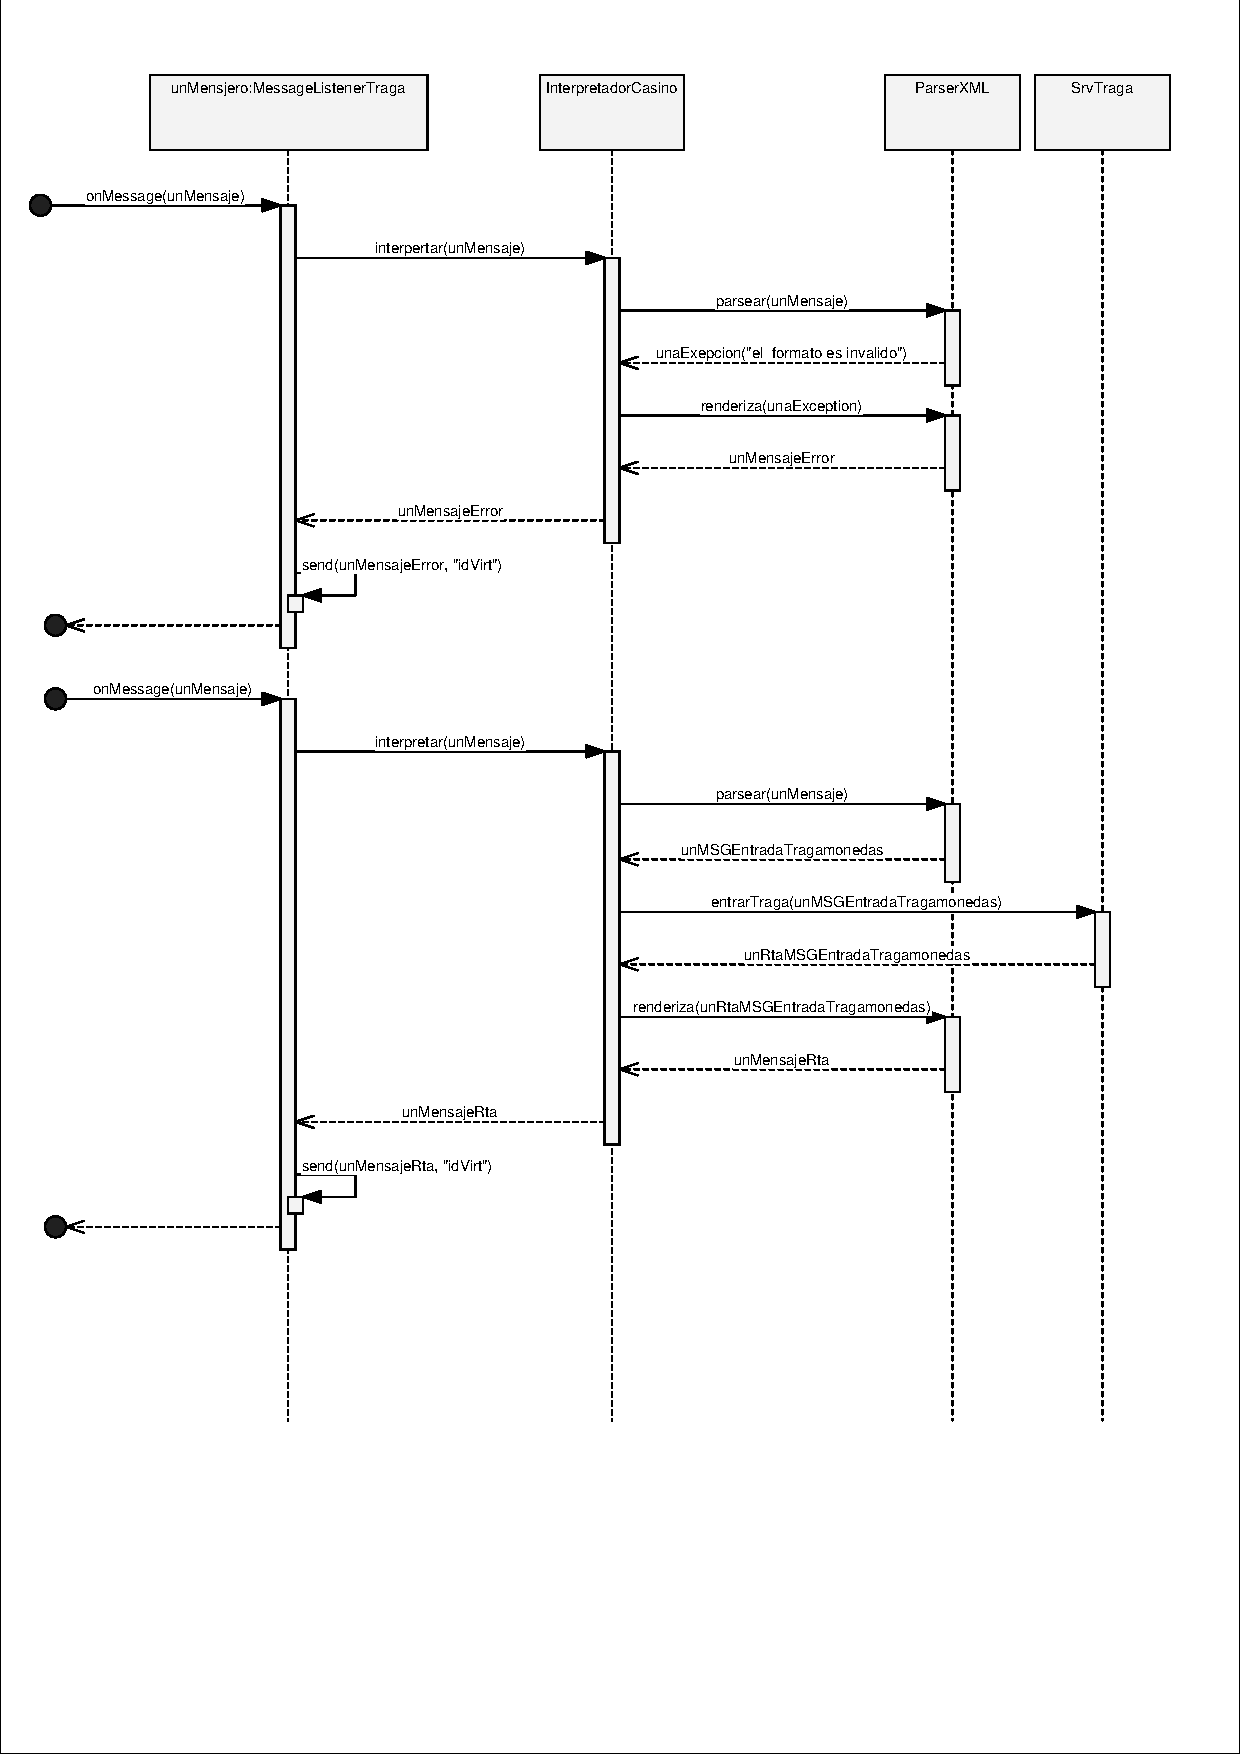
\includegraphics[scale=0.60]{mensajero.pdf}
%,angle=90]
%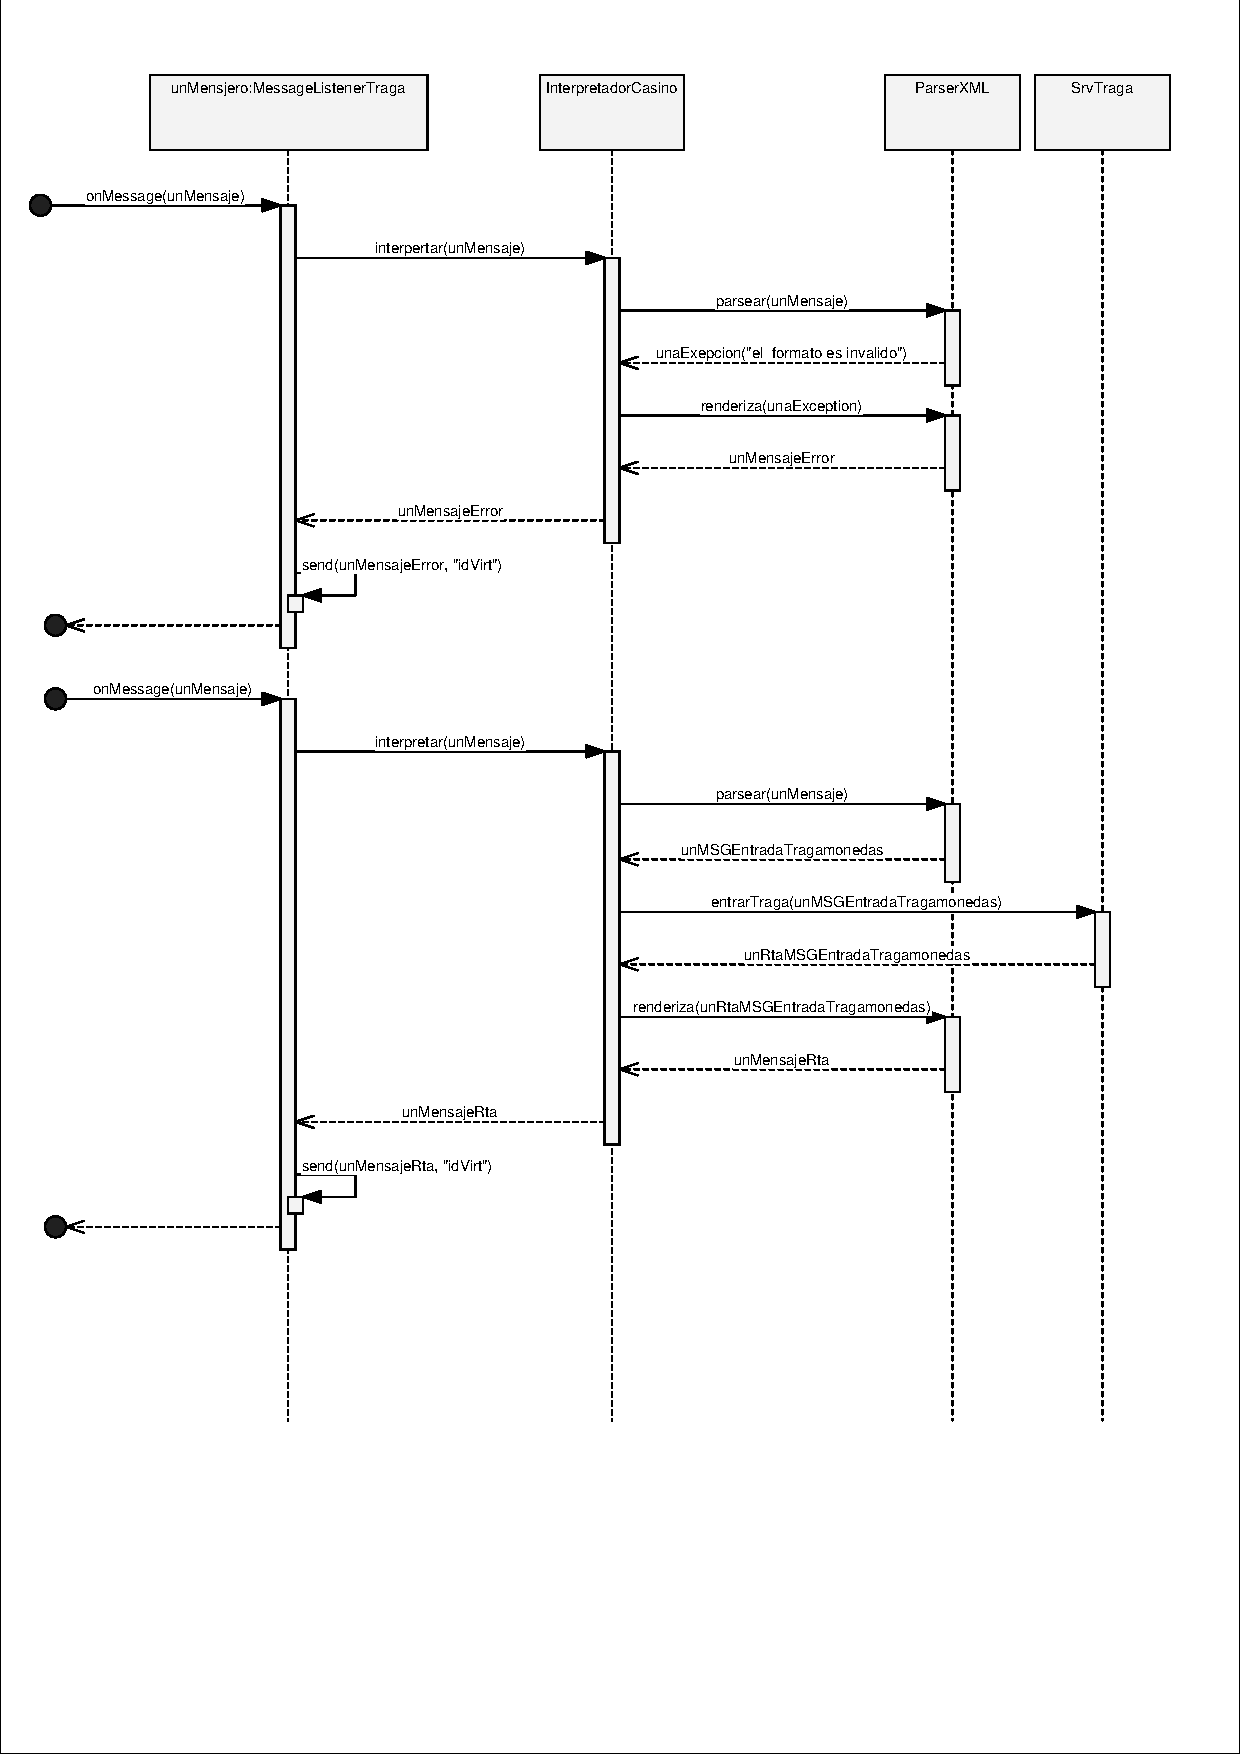
\includegraphics[height=4in,width=6in]{mensajero.pdf}
%  \includegraphics[height=60mm]{myfig.eps}
%  \includegraphics[scale=0.75]{myfig.eps}
%  \includegraphics[angle=45,width=52mm]{myfig.eps}


\end{document}


